\documentclass{article}
\usepackage{graphicx}
\usepackage[left=3.5cm, right = 3.5cm, top=3.5cm, bottom=3.5cm, head=13.6pt]{geometry}
\usepackage[onehalfspacing]{setspace}
\usepackage{amsthm}
\usepackage{amsmath}
\usepackage{amssymb}
\usepackage{mathtools}
\usepackage{float}
\usepackage{algpseudocode}
\usepackage{algorithm}
\usepackage{comment}
\usepackage{csquotes}
\usepackage{enumitem}


\title{Advanced Topics in Computer Graphics I - Sheet R04}
\author{Ninian Kaspers, Robin Landsgesell, Julian Stamm}
\date{\today}

\begin{document}

    \maketitle

    \section*{Assignment 2}
    
    In the right image a micro-facet BRDF was used.\\
    In the left image a Phong BRDF was used.\\

    \section*{Assignment 3}

    \begin{enumerate}[label=\alph*)]
        \item 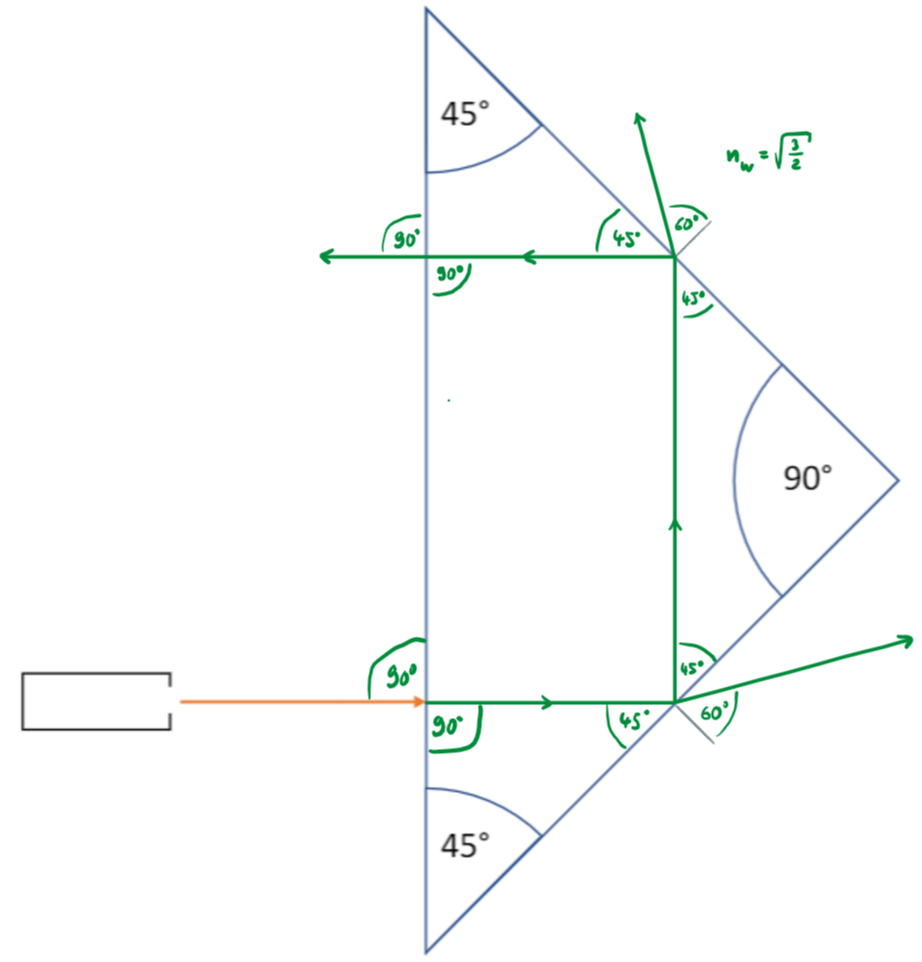
\includegraphics[width=0.5\textwidth]{3a.png}
        \item 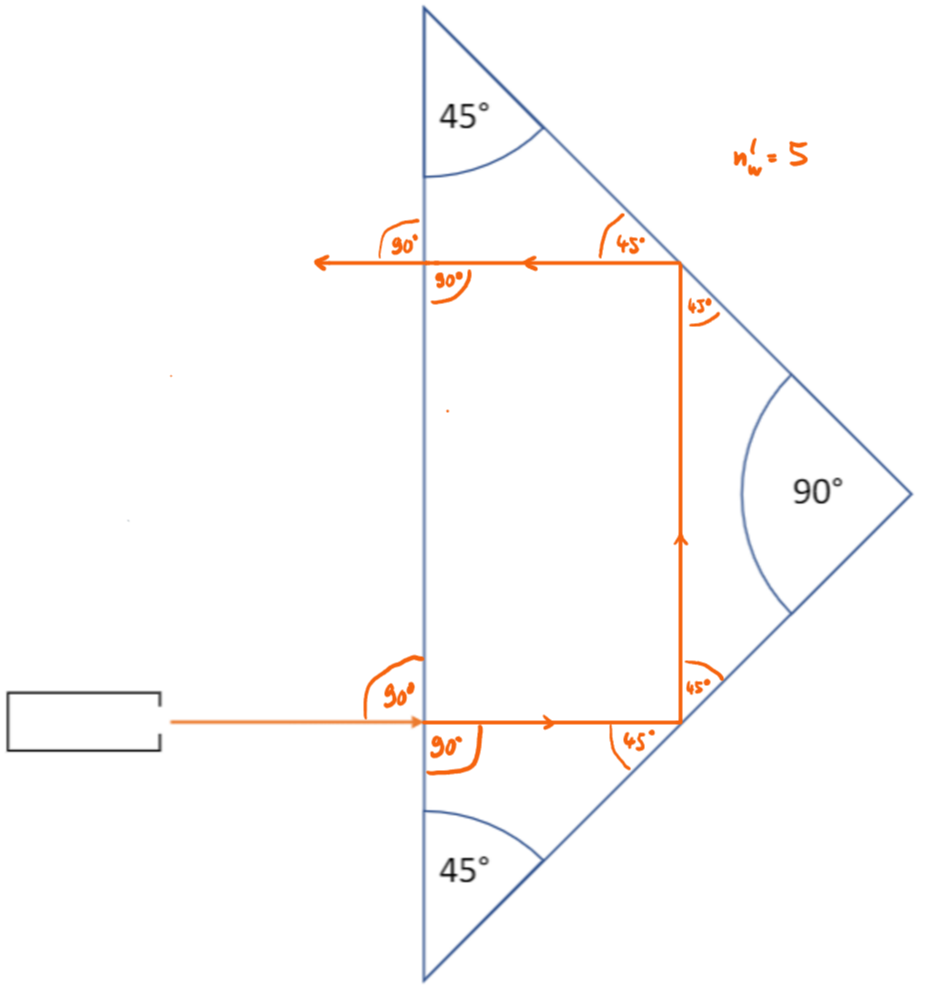
\includegraphics[width=0.5\textwidth]{3b.png}
        \item For b) the refractive index of the wedge was so high, that the light ray will not leave the wedge on the right side because of total internal reflection.
        \item $\hat{n}_w \sin(45^\circ) = n_a \sin(90^\circ) \Leftrightarrow \hat{n}_w = \sqrt{2}$ is the smallest refractive index leading to the same result.
    \end{enumerate}
    
\end{document}
